\documentclass[a4paper,12pt]{article}
\usepackage[T1]{fontenc}
\usepackage[utf8]{inputenc}
\usepackage{polski}
\usepackage{color}
\usepackage{graphicx}
\usepackage{amsmath}
\usepackage{amssymb}
\usepackage{hyperref}
\usepackage{float}
\usepackage{listings}
\usepackage[backend=biber]{biblatex}

\addbibresource{bibliografia.bib}

\lstset{
  basicstyle=\ttfamily,
  columns=flexible,
  keepspaces=true,
  showstringspaces=false,
  escapeinside={(*@}{@*)},
  literate={ą}{{\k{a}}}1
           {ć}{{\'{c}}}1
           {ę}{{\k{e}}}1
           {ł}{{\l{}}}1
           {ń}{{\'{n}}}1
           {ó}{{\'{o}}}1
           {ś}{{\'{s}}}1
           {ź}{{\'{z}}}1
           {ż}{{\.{z}}}1
           {Ą}{{\k{A}}}1
           {Ć}{{\'{C}}}1
           {Ę}{{\k{E}}}1
           {Ł}{{\L{}}}1
           {Ń}{{\'{N}}}1
           {Ó}{{\'{O}}}1
           {Ś}{{\'{S}}}1
           {Ź}{{\'{Z}}}1
           {Ż}{{\.{Z}}}1
           {"}{{\textquotedbl}}1
           {'}{{\textquotesingle}}1
           {`}{{\textasciigrave}}1
           {~}{{\textasciitilde}}1
           {^}{{\textasciicircum}}1
           {_}{{\textunderscore}}1
           {|}{{\textbar}}1
           {\{}{{\textbraceleft}}1
           {\}}{{\textbraceright}}1
           {[}{{[}}1
           {]}{{]}}1
}

\title{Zadanie - wykład 3}
\author{Mikołaj Kubś, 272662}
\date{\today}

\begin{document}

\maketitle

\begin{figure}[H]
	\centering
	
\includegraphics[width=1\textwidth]{images/task1.png}
	\caption{Opis zadań 1-3}
\end{figure}

\begin{figure}[H]
	\centering
	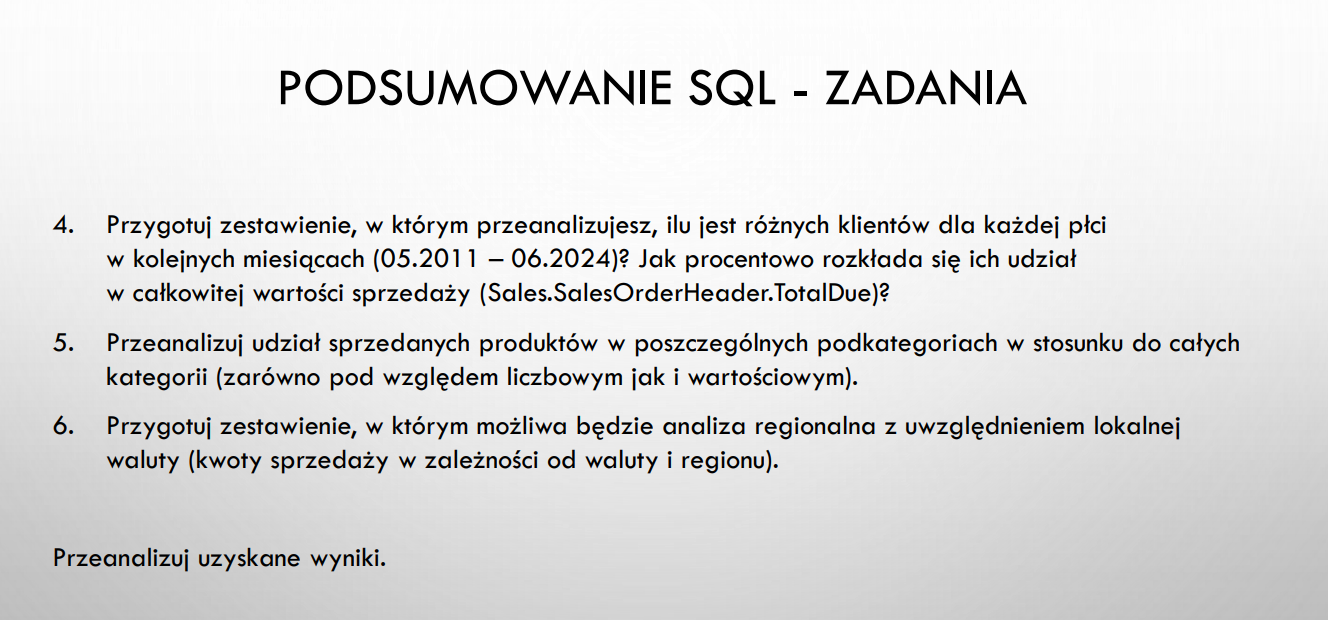
\includegraphics[width=1\textwidth]{images/task2.png}
	\caption{Opis zadań 4-6}
\end{figure}

\section{Kod kwerend 1-3}

\subsection{Kwerenda 1}

"Jaka była łączna suma transakcji (SalesOrderHeader.SubTotal) w poszczególnych latach dla kolejnych dni tygodnia?"

\begin{lstlisting}[
  language=SQL,
  showspaces=false,
  basicstyle=\ttfamily,
  numbers=left,
  numberstyle=\tiny,
  commentstyle=\color{green},
  tabsize=2
  ]
SET DATEFIRST 1;
SET LANGUAGE Polish;

SELECT 
  SUM(SubTotal) AS "Suma",
  DATENAME(DW, OrderDate) AS "Dzień tygodnia",
  DATEPART(YEAR, OrderDate) AS "Rok"
FROM Sales.SalesOrderHeader
GROUP BY 
  DATENAME(DW, OrderDate), 
  DATEPART(YEAR, OrderDate), 
  DATEPART(DW, OrderDate)
ORDER BY DATEPART(YEAR, OrderDate), DATEPART(DW, OrderDate)
\end{lstlisting}

\begin{figure}[H]
	\centering
	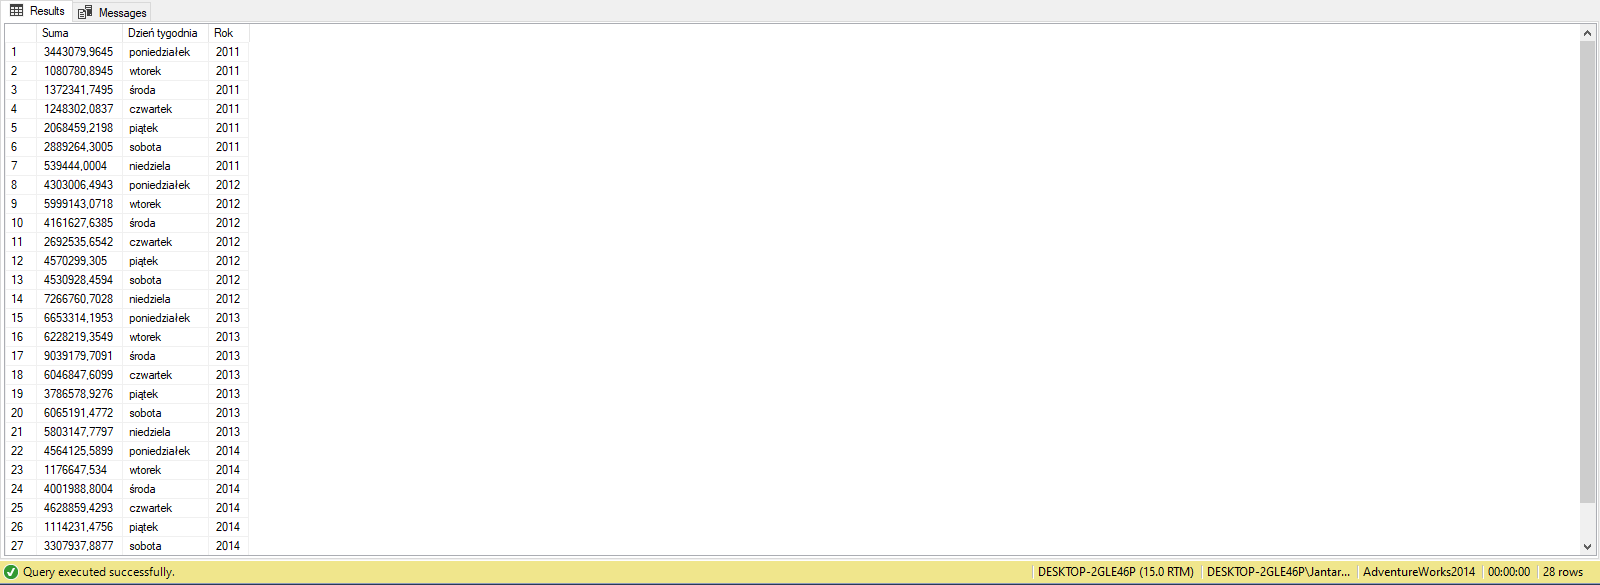
\includegraphics[width=1.0\textwidth]{images/1.png}
	\caption{Wyniki 1. kwerendy}
\end{figure}

W tym podpunkcie użycie CTE nie przyniosłoby korzyści.

\begin{figure}[H]
	\centering
	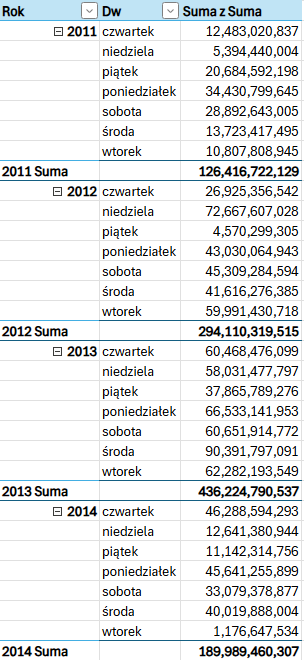
\includegraphics[width=0.4\textwidth]{images/1_excel.png}
	\caption{Tabela przestawna dla 1. kwerendy}
\end{figure}

Dla łatwiejszej analizy dodano tabelę przestawną.

W 2012 i 2013 roku suma roczna szybko rosła. 2014 rok się jeszcze nie skończył, co częściowo wyjaśnia niższą sumę dla 2014 roku.

W 2011 roku przychody w niedzielę były 2 razy niższe niż w drugim najgorszym dniu tygodnia tego roku. Poniedziałek był zdecydowanie najlepszy, a sobota druga.

W 2012 roku piątek był dniem bardzo niskich przychodów - suma była ponad 16 razy mniejsza niż dla najlepszego dnia, niedzieli.

W 2013 roku przychody były bardziej wyrównany, gdzie piątek (najsłabszy dzień) był ponad 2 razy mniej dochodowy niż najlepszy (środa).

W 2014 roku wtorek osiągnął bardzo niski wynik, prawie 40 razy niższy od najlepszego (czwartku).

Wnioskiem jest to, że różne dni w różnych latach odbiegają od normy dla danego roku. Jednak nie w każdym roku różnice były aż tak widoczne.

\subsection{Kwerenda 2}

"Zaproponuj podział klientów na 3 rozłączne grupy wiekowe. Ilu różnych klientów dokonało zakupów w kolejnych miesiącach roku w każdej z grup? Ilu klientów w poszczególnych grupach wykonało zakup dokładnie jeden raz?"

Zdecydowano się na podział klientów na 3 rozłączne grupy wiekowe o możliwie najrówniejszej liczbie członków. Do zrealizowania tego użyto funkcji "NTILE". Grupa 1 to najmłodsi, a 3 to najstarsi.

Zadanie dotyczy tak naprawdę dwóch kwerend.

\subsubsection{Ilu różnych klientów dokonało zakupów w kolejnych miesiącach roku w każdej z grup?}

Wersja z CTE:

{\small
\begin{lstlisting}[
	language=SQL,
	showspaces=false,
	basicstyle=\ttfamily,
	numbers=left,
	numberstyle=\tiny,
	commentstyle=\color{green},
	tabsize=2
]
WITH CustomerOrders AS (
	SELECT 
		Customer.CustomerID,
		NTILE(3) OVER (ORDER BY YEAR(GETDATE()) - YEAR(
			Person.Demographics.value(
				'declare default element namespace 
"http://schemas.microsoft.com/sqlserver/2004/07/adventure-works/IndividualSurvey";
(//BirthDate)[1]', 
				'DATE'
			)
		)) AS AgeGroup,
		YEAR(SalesOrderHeader.OrderDate) AS OrderYear
		MONTH(SalesOrderHeader.OrderDate) AS OrderMonth,
	FROM Sales.Customer AS Customer
	JOIN Person.Person AS Person ON Person.BusinessEntityID = Customer.PersonID
	JOIN 
		Sales.SalesOrderHeader AS SalesOrderHeader ON
			SalesOrderHeader.CustomerID = Customer.CustomerID
	WHERE
		Person.Demographics.exist(
			'declare default element namespace 
"http://schemas.microsoft.com/sqlserver/2004/07/adventure-works/IndividualSurvey";
(//BirthDate)[1]') = 1
)
SELECT
	OrderYear AS "Rok",
	OrderMonth AS "Miesiąc",
	AgeGroup AS "Grupa wiekowa", 
	COUNT(DISTINCT CustomerID) AS "Liczba unikalnych klientów"
FROM CustomerOrders
GROUP BY AgeGroup, OrderYear, OrderMonth
ORDER BY OrderYear, OrderMonth, AgeGroup
\end{lstlisting}}

Wersja bez CTE:

{\small
\begin{lstlisting}[
	language=SQL,
	showspaces=false,
	basicstyle=\ttfamily,
	numbers=left,
	numberstyle=\tiny,
	commentstyle=\color{green},
	tabsize=2
]
SELECT
    AgeGroup AS "Grupa wiekowa",
    OrderYear AS "Rok",
    OrderMonth AS "Miesiąc",
    COUNT(DISTINCT CustomerID) AS "Liczba unikalnych klientów"
FROM (
    SELECT 
        Customer.CustomerID,
        NTILE(3) OVER (ORDER BY YEAR(GETDATE()) - YEAR(
            Person.Demographics.value(
                'declare default element namespace 
"http://schemas.microsoft.com/sqlserver/2004/07/adventure-works/IndividualSurvey";
                (//BirthDate)[1]', 
                'DATE'
            )
        )) AS AgeGroup,
        YEAR(SalesOrderHeader.OrderDate) AS OrderYear,
        MONTH(SalesOrderHeader.OrderDate) AS OrderMonth
    FROM Sales.Customer AS Customer
    INNER JOIN Person.Person AS Person 
        ON Customer.PersonID = Person.BusinessEntityID
    INNER JOIN Sales.SalesOrderHeader AS SalesOrderHeader 
        ON Customer.CustomerID = SalesOrderHeader.CustomerID
    WHERE Person.Demographics.exist(
        'declare default element namespace 
"http://schemas.microsoft.com/sqlserver/2004/07/adventure-works/IndividualSurvey";
        (//BirthDate)[1]') = 1
) AS CustomerOrderData
GROUP BY AgeGroup, OrderYear, OrderMonth
ORDER BY OrderYear, OrderMonth, AgeGroup
\end{lstlisting}}

\begin{figure}[H]
	\centering
	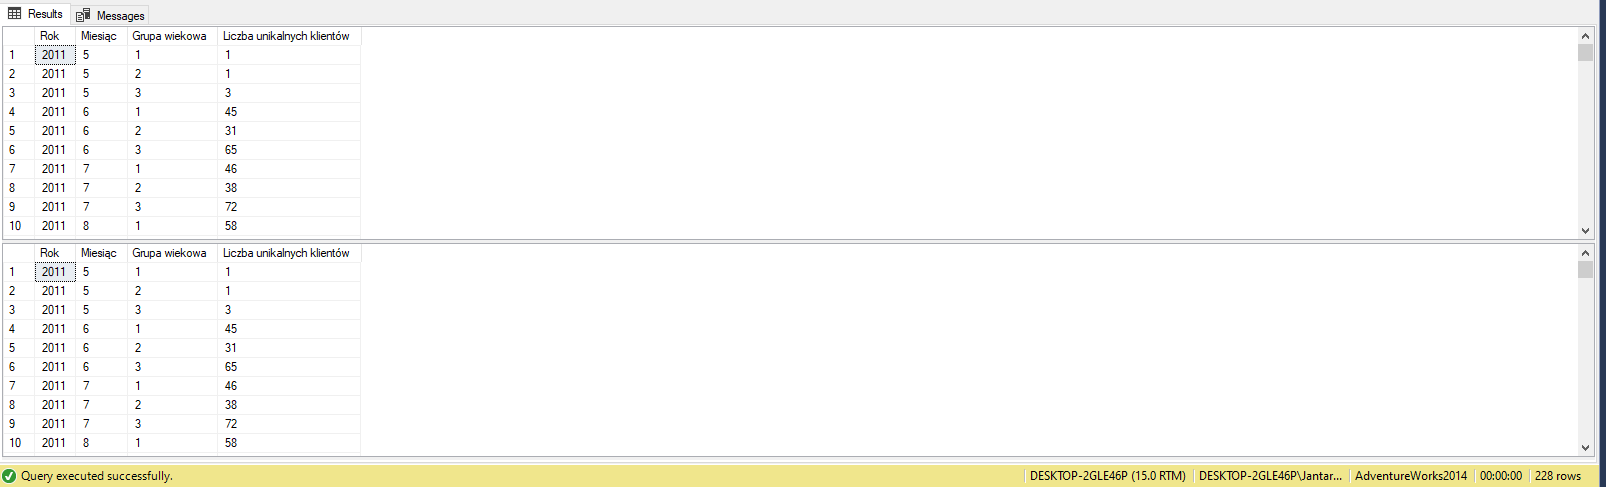
\includegraphics[width=0.4\textwidth]{images/2.png}
	\caption{Wyniki 2. kwerendy}
\end{figure}

Wersja "bez" CTE i z nim są bardzo podobne. Nie da się przenieść bezpośrednio NTILE'a i reszty logiki do jednego zapytania bez wcześniejszego wyliczenia grup wiekowych, ponieważ nie da się pogrupować po funkcji okienkowej. Nielogiczne byłoby naraz grupowanie i wybieranie. Jednym ze sposobów rozwiązania tego problemu mogłoby być wyliczenie wcześniej górnej granicy wieku dla 1. i 2. grupy, a następnie przypisanie klientów i grupowanie w jednym zapytanie - nadal trzeba jednak coś wyliczyć wcześniej.

W większości miesięcy liczba unikalnych klientów jest względnie podobna do siebie dla każdej grupy. Zdarza się, że najliczniejsza grupa jest 2-3 razy liczniejsza od tej najmniej licznej w danym miesiącu. Często się potem w tym samym roku zdarza odwrotna sytuacja. W 2012 roku najmłodsza grupa jest najliczniejsza, a w 2014 najmniej liczna o dość podobną liczbę osób.

\begin{figure}[H]
	\centering
	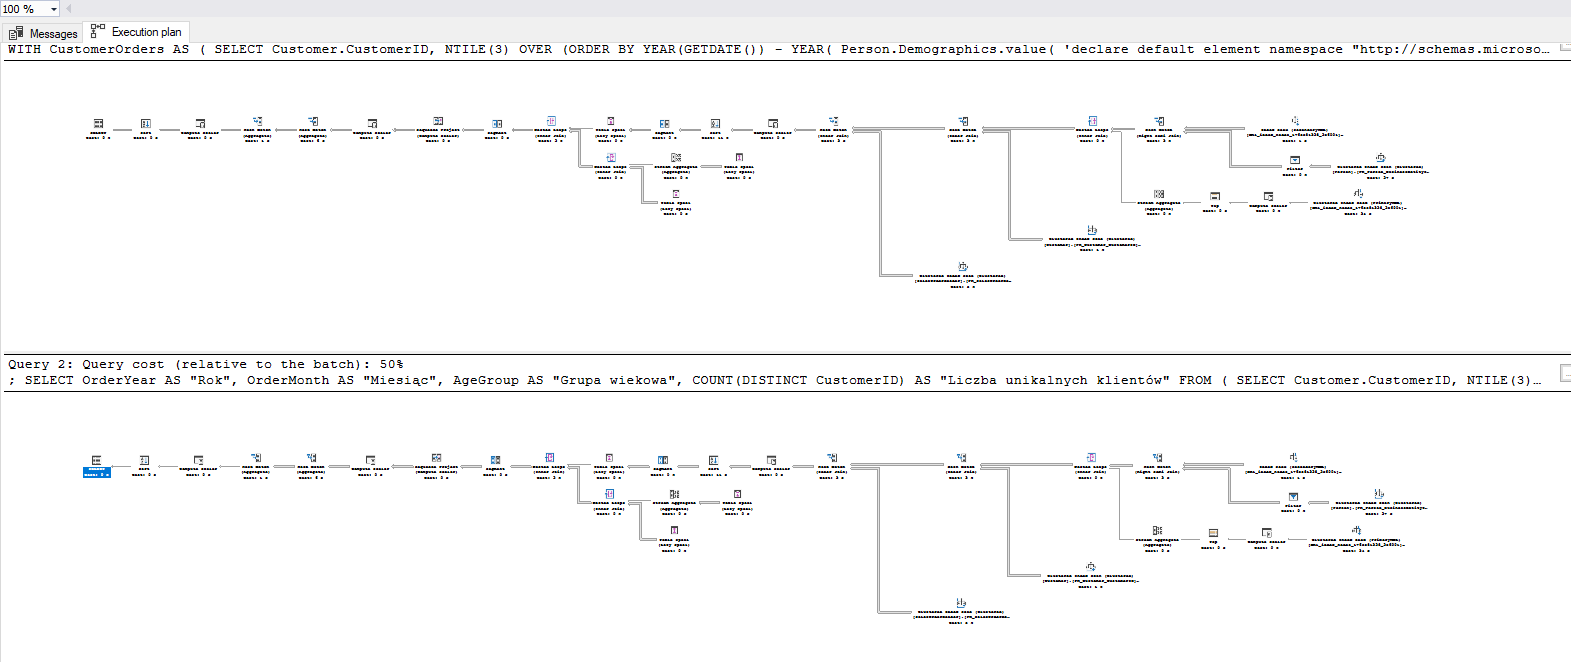
\includegraphics[width=0.4\textwidth]{images/2_execution_plan.png}
	\caption{Porównanie execution plan}
\end{figure}

Obie kwerendy działają tak samo z wcześniej opisanych powodów.

\subsubsection{Ilu klientów w poszczególnych grupach wykonało zakup dokładnie jeden raz?}

Wersja z CTE:

{\small
\begin{lstlisting}[
	language=SQL,
	showspaces=false,
	basicstyle=\ttfamily,
	numbers=left,
	numberstyle=\tiny,
	commentstyle=\color{green},
	tabsize=2
]
WITH OrdersWithCustomerDetails AS (
    SELECT 
        Customer.CustomerID,
        NTILE(3) OVER (ORDER BY YEAR(GETDATE()) - YEAR(
            Person.Demographics.value(
                'declare default element namespace 
"http://schemas.microsoft.com/sqlserver/2004/07/adventure-works/IndividualSurvey";
                (//BirthDate)[1]', 
                'DATE'
            )
        )) AS AgeGroup,
        SalesOrderHeader.SalesOrderID,
        YEAR(SalesOrderHeader.OrderDate) AS OrderYear,
        MONTH(SalesOrderHeader.OrderDate) AS OrderMonth
    FROM Sales.Customer AS Customer
    INNER JOIN Person.Person AS Person
        ON Customer.PersonID = Person.BusinessEntityID
    INNER JOIN Sales.SalesOrderHeader AS SalesOrderHeader
        ON Customer.CustomerID = SalesOrderHeader.CustomerID
    WHERE Person.Demographics.exist(
        'declare default element namespace 
"http://schemas.microsoft.com/sqlserver/2004/07/adventure-works/IndividualSurvey";
        (//BirthDate)[1]') = 1
),
CustomersWithSingleOrder AS (
    SELECT
        CustomerID,
        AgeGroup
    FROM OrdersWithCustomerDetails
    GROUP BY CustomerID, AgeGroup
    HAVING COUNT(SalesOrderID) = 1
)
SELECT
    AgeGroup AS "Grupa wiekowa",
    COUNT(CustomerID) AS "Liczba klientów z pojedynczym zamówieniem"
FROM CustomersWithSingleOrder
GROUP BY AgeGroup
ORDER BY AgeGroup
\end{lstlisting}}

Wersja bez CTE:

{\small
\begin{lstlisting}[
	language=SQL,
	showspaces=false,
	basicstyle=\ttfamily,
	numbers=left,
	numberstyle=\tiny,
	commentstyle=\color{green},
	tabsize=2
]
SELECT
    CustomerAgeGroup AS "Grupa wiekowa",
    COUNT(*) AS "Liczba klientów z jednym zamówieniem"
FROM (
    SELECT 
        CustomerID,
        CustomerAgeGroup
    FROM (
        SELECT 
            SalesCustomer.CustomerID,
            NTILE(3) OVER (ORDER BY YEAR(GETDATE()) - YEAR(
                PersonTable.Demographics.value(
                    'declare default element namespace 
"http://schemas.microsoft.com/sqlserver/2004/07/adventure-works/IndividualSurvey";
                    (//BirthDate)[1]', 
                    'DATE'
                )
            )) AS CustomerAgeGroup,
            SalesOrderHeader.SalesOrderID
        FROM Sales.Customer AS SalesCustomer
        INNER JOIN Person.Person AS PersonTable 
            ON SalesCustomer.PersonID = PersonTable.BusinessEntityID
        INNER JOIN Sales.SalesOrderHeader AS SalesOrderHeader 
            ON SalesCustomer.CustomerID = SalesOrderHeader.CustomerID
        WHERE PersonTable.Demographics.exist(
            'declare default element namespace 
"http://schemas.microsoft.com/sqlserver/2004/07/adventure-works/IndividualSurvey";
            (//BirthDate)[1]'
        ) = 1
    ) AS OrdersPerCustomer
    GROUP BY CustomerID, CustomerAgeGroup
    HAVING COUNT(SalesOrderID) = 1
) AS SingleOrderCustomers
GROUP BY CustomerAgeGroup
ORDER BY CustomerAgeGroup
\end{lstlisting}}

\begin{figure}[H]
	\centering
	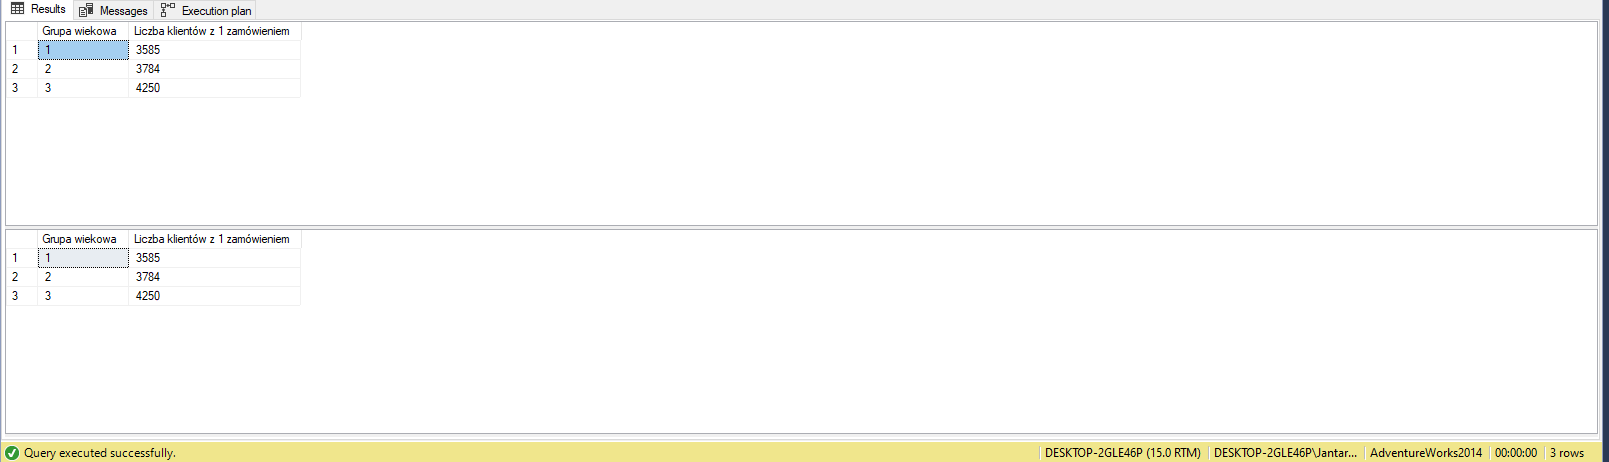
\includegraphics[width=1.0\textwidth]{images/2.1.png}
	\caption{Wyniki 2. kwerendy, część 2.}
\end{figure}

Wersja "bez" CTE i z CTE są bardzo podobne, z powodów opisanych wcześniej, dla pierwszej kwerendy w zadaniu 2. Dużym błędem byłoby tutaj wyliczenie najpierw klientów z jedną transakcją, a potem grupowanie ich NTILE'm na podstawie wyniku - NTILE wtedy analizowałby tylko wycinek całej populacji

Liczba klientów z jedną transakcją jest względnie podobna dla każdej grupy klientów. Najwięcej najstarszych klientów kupiło coś tylko raz. Najmniej młodych dokonało zakupu tylko raz.

\begin{figure}[H]
	\centering
	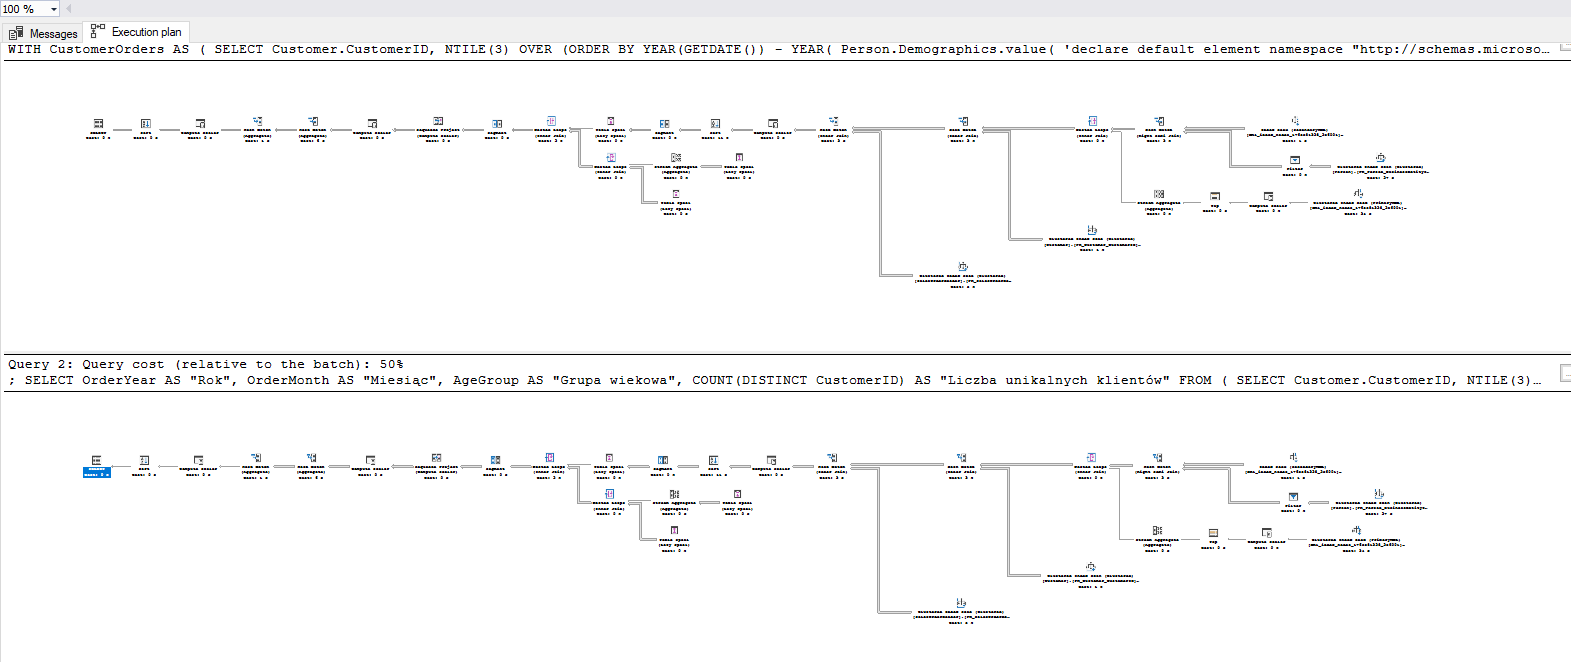
\includegraphics[width=0.4\textwidth]{images/2_execution_plan.png}
	\caption{Porównanie execution plan}
\end{figure}

Obie kwerendy działają tak samo z wcześniej opisanych powodów.

\subsection{Kwerenda 3}

"Przygotuj zestawienie produktów, których sprzedaje się miesięcznie min. 20 sztuk. Dla każdego produktu podaj jego kategorię"

Kwerenda z CTE:

{\small
\begin{lstlisting}[
	language=SQL,
	showspaces=false,
	basicstyle=\ttfamily,
	numbers=left,
	numberstyle=\tiny,
	commentstyle=\color{green},
	tabsize=2
]
WITH ProductCategories AS (
    SELECT 
        ProductSubcategory.ProductSubcategoryID,
        ProductCategory.Name AS CategoryName
    FROM Production.ProductSubcategory
    JOIN Production.ProductCategory 
        ON ProductSubcategory.ProductCategoryID = ProductCategory.ProductCategoryID
),
MonthlySales AS (
    SELECT 
        Product.ProductID,
        Product.ProductSubcategoryID,
        Product.Name AS ProductName,
        YEAR(SalesOrderHeader.OrderDate) AS SalesYear,
        MONTH(SalesOrderHeader.OrderDate) AS SalesMonth,
        COUNT(*) AS MonthlyCount
    FROM Sales.SalesOrderDetail AS SalesDetail
    JOIN Production.Product AS Product 
        ON SalesDetail.ProductID = Product.ProductID
    JOIN Sales.SalesOrderHeader AS SalesOrderHeader
        ON SalesDetail.SalesOrderID = SalesOrderHeader.SalesOrderID
    GROUP BY 
        Product.ProductID, 
        Product.ProductSubcategoryID,
        Product.Name, 
        YEAR(SalesOrderHeader.OrderDate), 
        MONTH(SalesOrderHeader.OrderDate)
),
SalesWithCategory AS (
    SELECT 
        MonthlySales.ProductID,
        MonthlySales.ProductName,
        ProductCategories.CategoryName,
        MonthlySales.SalesYear,
        MonthlySales.SalesMonth,
        MonthlySales.MonthlyCount
    FROM MonthlySales
    LEFT JOIN ProductCategories 
        ON MonthlySales.ProductSubcategoryID = 
				ProductCategories.ProductSubcategoryID
),
ProductsWithMinSales AS (
    SELECT 
        ProductID,
        ProductName,
        CategoryName
    FROM SalesWithCategory
    GROUP BY ProductID, ProductName, CategoryName
    HAVING MIN(MonthlyCount) >= 20
)
SELECT 
    SalesWithCategory.ProductName,
    SalesWithCategory.CategoryName,
    SalesWithCategory.SalesYear,
    SalesWithCategory.SalesMonth,
    SalesWithCategory.MonthlyCount
FROM SalesWithCategory
JOIN ProductsWithMinSales 
    ON SalesWithCategory.ProductID = ProductsWithMinSales.ProductID
ORDER BY 
	SalesWithCategory.ProductName, 
	SalesWithCategory.SalesYear, 
	SalesWithCategory.SalesMonth;
\end{lstlisting}}

Kwerenda bez CTE:

{\small
\begin{lstlisting}[
	language=SQL,
	showspaces=false,
	basicstyle=\ttfamily,
	numbers=left,
	numberstyle=\tiny,
	commentstyle=\color{green},
	tabsize=2
]
SELECT 
    Sales.ProductName,
    Sales.CategoryName,
    Sales.SalesYear,
    Sales.SalesMonth,
    Sales.MonthlyCount
FROM (
    SELECT 
        Product.ProductID,
        Product.Name AS ProductName,
        ProductCategory.Name AS CategoryName,
        YEAR(SalesOrderHeader.OrderDate) AS SalesYear,
        MONTH(SalesOrderHeader.OrderDate) AS SalesMonth,
        COUNT(*) AS MonthlyCount
    FROM Sales.SalesOrderDetail AS SalesDetail
    JOIN Production.Product AS Product 
        ON SalesDetail.ProductID = Product.ProductID
    JOIN Sales.SalesOrderHeader AS SalesOrderHeader
        ON SalesDetail.SalesOrderID = SalesOrderHeader.SalesOrderID
    LEFT JOIN Production.ProductSubcategory AS ProductSubcategory
        ON Product.ProductSubcategoryID = ProductSubcategory.ProductSubcategoryID
    LEFT JOIN Production.ProductCategory AS ProductCategory
        ON ProductSubcategory.ProductCategoryID = ProductCategory.ProductCategoryID
    GROUP BY 
        Product.ProductID, 
        Product.Name,
        ProductCategory.Name,
        YEAR(SalesOrderHeader.OrderDate), 
        MONTH(SalesOrderHeader.OrderDate)
) AS Sales
WHERE Sales.ProductID IN (
    SELECT ProductID
    FROM (
        SELECT 
            Product.ProductID,
            COUNT(*) AS MonthlyCount
        FROM Sales.SalesOrderDetail AS SalesDetail
        JOIN Production.Product AS Product 
            ON SalesDetail.ProductID = Product.ProductID
        JOIN Sales.SalesOrderHeader AS SalesOrderHeader
            ON SalesDetail.SalesOrderID = SalesOrderHeader.SalesOrderID
        GROUP BY 
            Product.ProductID,
            YEAR(SalesOrderHeader.OrderDate), 
            MONTH(SalesOrderHeader.OrderDate)
    ) AS Monthly
    GROUP BY ProductID
    HAVING MIN(MonthlyCount) >= 20
)
ORDER BY Sales.ProductName, Sales.SalesYear, Sales.SalesMonth;
\end{lstlisting}}

\begin{figure}[H]
	\centering
	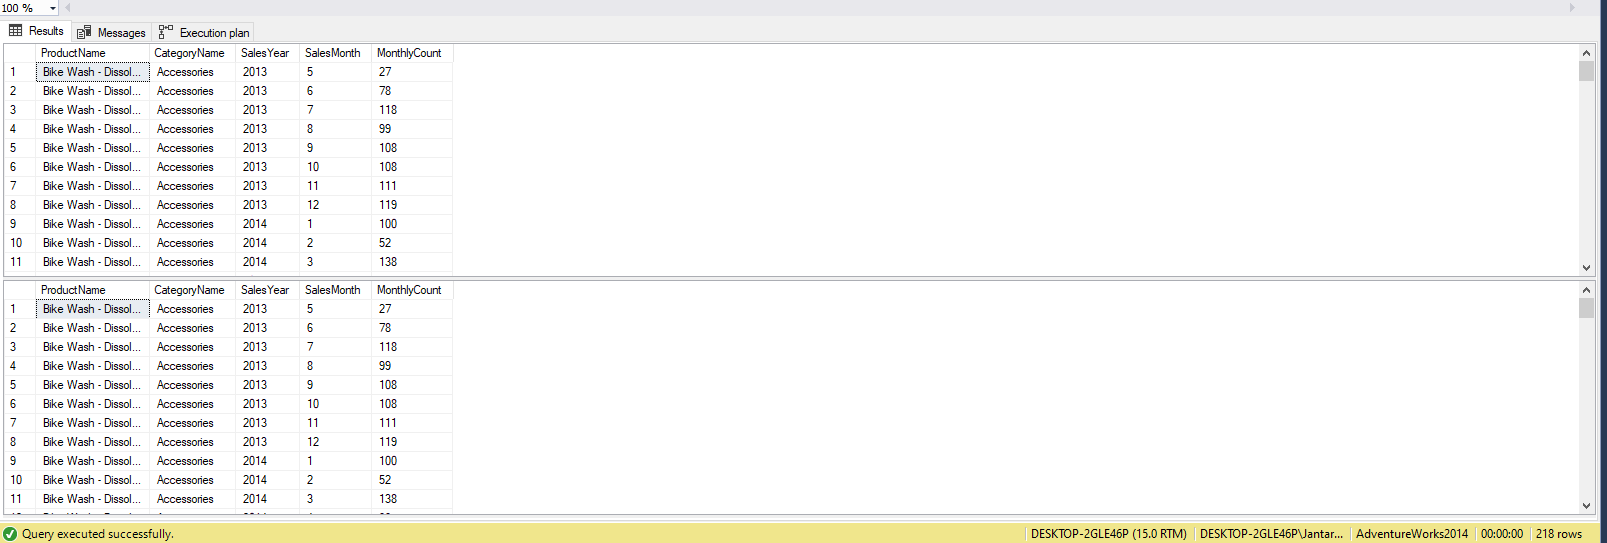
\includegraphics[width=1.0\textwidth]{images/3.png}
	\caption{Wyniki 3. kwerendy}
\end{figure}

Nie ma wielu produktów, które konsekwentnie sprzedają się miesięcznie w liczbie ponad 20 sztuk. Takich produktów jest 8 - 6 z kategorii akcesorium, a 2 z kategorii rowery. Wszystkie te produkty zostały po raz pierwszy zakupione w maju 2013 roku. Jak wiadomo z innych analiz, w połowie 2013 roku sprzedaż sklepu znacznie się zwiększyła, co prawdopodobnie wywołało taki stan rzeczy. Były inne produkty, np. "AWC Logo Cap", które utrzymywały wysoką sprzedaż przez 4 lata - niestety wystarczyły dwa gorsze miesiące i nie znalazł się wśród wyników.

Wniosek jest taki, że kwerenda z tak sztywnymi zasadami może wykluczyć inne produkty-sukcesy.

\begin{figure}[H]
	\centering
	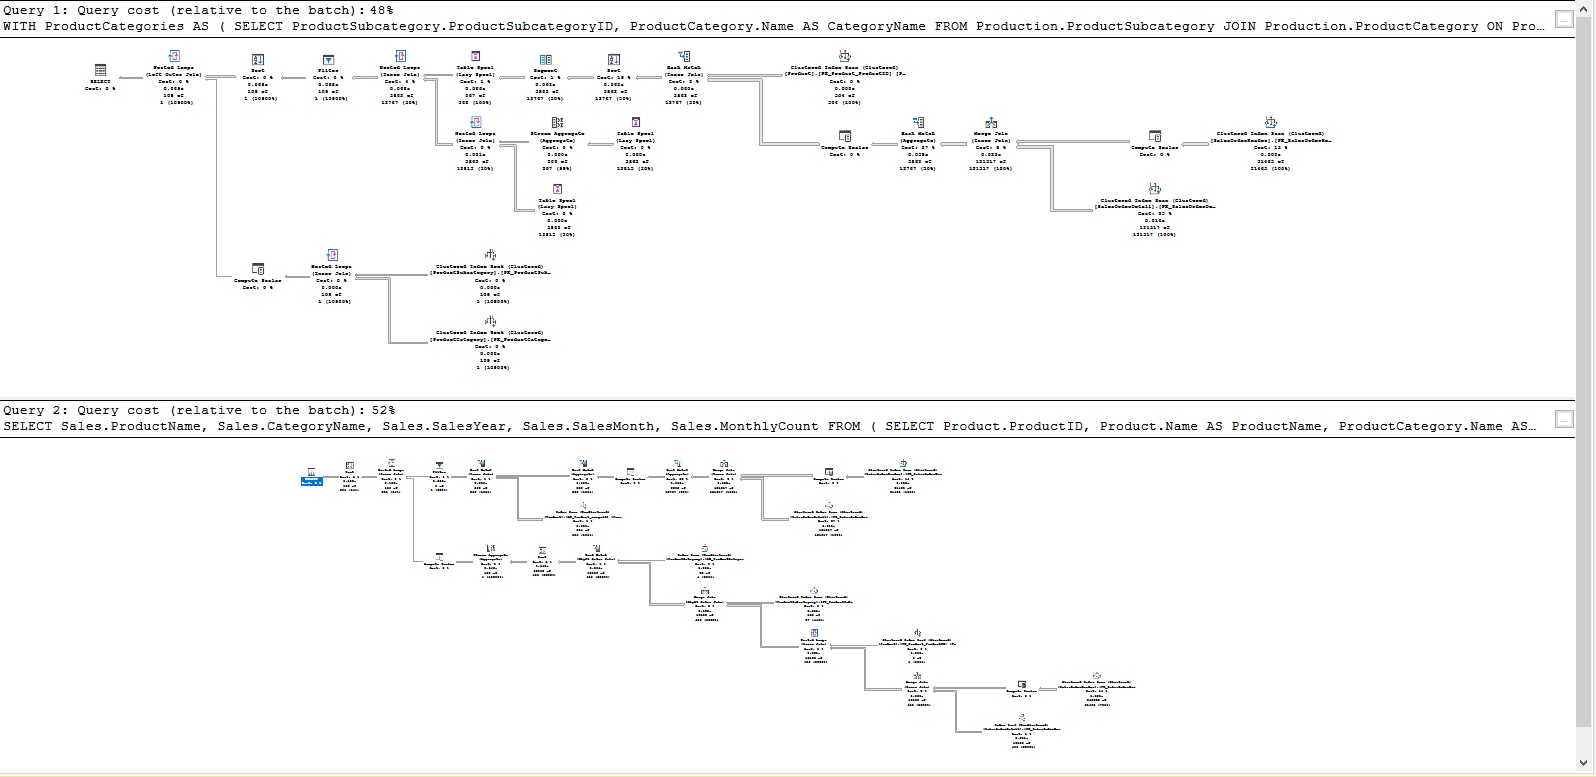
\includegraphics[width=1.0\textwidth]{images/3_execution_plan.png}
	\caption{Porównanie exeuction plan}
\end{figure}

Wersja z CTE jest tylko nieznacznie szybsza - 52\% do 48\%.

\end{document}